\documentclass[12pt, titlepage]{article}
\title{PWS AI}
\author{Maarten Stremler \and Ivar de Bruin \and Jaap de Jong}

\PassOptionsToPackage{hyphens}{url}
\usepackage{amssymb, amsmath}
\usepackage{hyperref}
\usepackage{listings}
\usepackage{color}
\usepackage{tikz}
\usepackage[utf8]{inputenc}
\usepackage[T1]{fontenc}
\usepackage{enumitem}

%forces a pagebreak before a new section
\let\oldsection\section
\renewcommand\section{\clearpage\oldsection}

%defines the look of the code used
\definecolor{dkgreen}{rgb}{0,0.6,0}
\definecolor{gray}{rgb}{0.5,0.5,0.5}
\definecolor{mauve}{rgb}{0.58,0,0.82}

%how the code will look.
\lstset{frame=tb,
	language=Java,
	aboveskip=3mm,
	belowskip=3mm,
	showstringspaces=false,
	columns=flexible,
	basicstyle={\small\ttfamily},
	numbers=none,
	numberstyle=\tiny\color{gray},
	keywordstyle=\color{blue},
	commentstyle=\color{dkgreen},
	stringstyle=\color{mauve},
	breaklines=true,
	breakatwhitespace=true,
	tabsize=3
}

\setlength{\parindent}{0pt}
%No tabs in the first line of a new paragraph
\setlength{\parskip}{\baselineskip}
%Automatic whiteline between paragraphs

%used for pictures
\tikzset{%
	every neuron/.style={
		circle,
		draw,
		minimum size=1cm
	},
	neuron missing/.style={
		draw=none,
		scale=4,
		text height=0.333cm,
		execute at begin node=\color{black}$\vdots$
	},
}


\begin{document}
	\begin{titlepage} % Suppresses headers and footers on the title page
		
		\centering % Centre everything on the title page
		
		\scshape % Use small caps for all text on the title page
		
		\vspace*{\baselineskip} % White space at the top of the page
		
		%------------------------------------------------
		%	Title
		%------------------------------------------------
		
		\rule{\textwidth}{1.6pt}\vspace*{-\baselineskip}\vspace*{2pt} % Thick horizontal rule
		\rule{\textwidth}{0.4pt} % Thin horizontal rule
		
		\vspace{0.75\baselineskip} % Whitespace above the title
		
		{\LARGE Facial recognition\\ MAN VS AI\\} % Title
		
		\vspace{0.75\baselineskip} % Whitespace below the title
		
		\rule{\textwidth}{0.4pt}\vspace*{-\baselineskip}\vspace{3.2pt} % Thin horizontal rule
		\rule{\textwidth}{1.6pt} % Thick horizontal rule
		
		\vspace{2\baselineskip} % Whitespace after the title block
		
		%------------------------------------------------
		%	Subtitle
		%------------------------------------------------
		
		Profiel werkstuk documentatie % Subtitle or further description
		
		\vspace*{3\baselineskip} % Whitespace under the subtitle
		
		%------------------------------------------------
		%	Editor(s)
		%------------------------------------------------
		
		Edited By
		
		\vspace{0.5\baselineskip} % Whitespace before the editors
		
		{\scshape\Large Ivar de Bruin \\ Maarten Stremler \\ Jaap de Jong \\} % Editor list
		
		\vspace{0.5\baselineskip} % Whitespace below the editor list
		
		\textit{Guido de Brès \\ Wartburg College} % Editor affiliation
		
		\vfill % Whitespace between editor names and publisher logo
		
		%------------------------------------------------
		%	Publisher
		%------------------------------------------------
		
		\vspace{0.3\baselineskip} % Whitespace under the publisher logo
		
		2017 % Publication year
		
	\end{titlepage}
	\tableofcontents
	
	\section{Introduction}
	In recent years, there have been enormous advances in the field of AI. In 2016 Google's DeepMind AI beat the reigning world champion at Go, one of the most difficult games there is\cite{byford16}. Go has a possibility space which is exponentially larger than that of, for instance, chess. In the same year it was announced that Microsoft had built an AI which surpassed humans when it came to speech recognition.
	Most, if not all, of these huge steps forward have been made possible due to an exponential rise in computing power and the usage of GPUs for massive parallel computing in the last few years.
	\\
	\\
	Another very important factor is the revival of the neural net. This particular form of AI was devised in the late forties. In the seventies they fell out of grace, but with the advance of computing power, so called ‘deep’ neural networks became feasible and ever since 2010, neural networks have dominated the field of AI.\cite{kuzovkin16}\cite{foote17} Artificial Intelligence usually makes headlines when it has beaten us humans in something. Often it is a board game or some other type of game. Because of this constant comparison between humans and AI, we wanted to compare them on another level. An essential function of the human brain is recognizing people's faces. This is, among other things, very important in social life. Because of that, this research will focus on facial recognition by AI.
	
	\subsection{Main Question}
	The main goal of this research is to answer the following question:
	\begin{center}
		\textit{What is the difference in speed and effectivity between humans and artificial 					intelligence, when it comes to facial recognition?}
	\end{center}
	
	\subsection{Demarcation}
	For this research, an AI capable of recognizing faces will be built and tested against human intelligence. This will be done by giving the AI and one of the researchers a fixed amount of time to classify as many pictures of human faces as possible. After the time is over, speed (how many pictures were processed) and effectiveness (what part of the processed pictures has been classified correctly) will be measured, in order to evaluate the performance of both the AI and its human counterpart.
	
	\subsubsection{Specificity}
	The concepts discussed in the main question are very described in a specific manner. It should, however be remarked that the term 'Artificial Intelligence' is not very specific, because the exact structure of the AI is not yet known at this moment. 
	
	\subsubsection{Measurability}
	The performance of the AI and the human test subjects will be measured by giving them a certain amount of tests. The amount of correct and incorrect answers will be logged and, if relevant, the amount of time the subject needs to finish the test will be as well. After that, the AI could possibly be trained for other tasks, such as playing chess. Just like facial recognition there are a lot of different methods to compare performance between human and AI here as well.
	
	\subsubsection{Acceptability}
	There is enough time to design and build the AI. Researches can program at home and at school. The training of the AI can be paused without corrupting any data, so the AI can be trained with big data sets without having to let a computer run ceaselessly for a certain amount of days. Running an AI is not dangerous for the computer or the network.
	
	\subsubsection{Realistic}
	Researchers possess enough mathematical and programming knowledge to build the AI. There is still some uncertainty about the time needed to build a working AI.
	
	\subsubsection{Time-bound}
	The duration of a test is not of interest, as long as human and AI get the same amount of time to finish the test. It is assumed that this will be done fairly quickly. The goal is, to build a relatively fast AI that should outperform humans, at least when looking at the time required to recognize someone. The designing, building and testing of the AI, however, is very likely to require a lot more time.
	
	
	\section{Sub-questions}
	\begin{enumerate}[align=left, font=\large]
		\item [2.1] {There are lots of different ways of building neural networks and there are lots of hyper-parameters to configure. Which type of neural network works best for the purpose of this research?
			\item [2.2] How does one actually implement an AI capable of facial recognition?
			\item[2.3] What can be said about the differences between humans and AI when it comes to mastering certain tasks?
			\begin{enumerate}[font=\normalsize]
				\item[2.3.1] What is the difference in time required to master a certain task?
				\item[2.3.2] What is the difference when it comes to the amount of examples required to master a certain task?
			\end{enumerate}
			\item[2.4] What is the difference in performance between humans and AI?
			\begin{enumerate}[font=\normalsize]
				\item[2.4.1] What is the difference when it comes to the amount of successfully recognized images?
				\item[2.4.2] Are humans or AI better at recognizing linking pictures of people at different ages, or which 'system' is more sensitive when it comes to the aging process?
			\end{enumerate}
			\item[2.5] Can an AI capable of facial recognition also be trained to perform other tasks?
			\begin{enumerate}[font=\normalsize]
				\item[2.5.1]How can it crack Captchas and how does it need to be improved to do so?
				\item[2.5.2] How can it play simple board games and how does it need to be improved to do so?
				\item[2.5.3] Is it possible for the AI to differentiate between different kinds of input, so that one and the same AI is capable of performing multiple tasks?
			\end{enumerate}
			\item[2.6] Even if the AI has a lower success rate recognizing faces on pictures, it will probably still be way faster than the average human. In which situations would this advantage of being fast be of such importance, that the disadvantage when it comes to accuracy can be neglected?
		\end{enumerate}
		
		\section{Research method}
		
		\subsection{Literature research as preparation for building the AI}
		Lots of reliable sources were found stating that convolutional neural nets are the state of the art when it comes to image recognition\cite{gu}\cite{imageRecognition17}. In fact, no reseach was found on computer vision which didn't include something about neural nets. This is why neural nets will be the AI technique used and why the focus of the literature research is going to lie on the specifics of the neural net which will be built..
		
		\bigskip
		Information about neural nets will come mainly from YouTube and sources mentioned in relevant Wikipedia articles (about e.g. backpropagation), though there are also a few blogs containing very valuable information on the back propagation algorithm. Books and research articles on neural nets usually don't provide any information needed for actually building and training neural nets, but rather information on the best activation functions, new complicated ways to better train neural nets and so on. This is all very interesting when one is trying to improve an existing neural net or when one has a lot of experience building neural nets, but when making a first-time build, all this extra information isn't really needed.
		
		\subsection{Comparing the AI to humans}
		After an AI has been built which is able to compare pairs of pictures and tell us whether they are of the same person or not, a series of tests and experiments will be conducted in order to compare the AI to humans and to test the limitations of the AI. The research will be experimental.
		
		When comparing humans to AI, it should not be forgotten that the strengths of AI are different to those of humans. Therefore, it is best to conduct a wide range of tests, looking at different aspects of facial recognition.
		
		Only the first two tests are real tests of the AI, comparing it to humans. Test 3 and test 4 simply state that the first two tests will be conducted on different people, different AIs and with multiple different samples in such way that other properties of the AI can be researched. The four tests are quantitative in nature, while the two experiments lean toward the qualitative side.
		
		Finally, there are two experiments which can be conducted on a working facial recognition AI. All of the research will be done using the observational method. There are also some existing data sets (pictures of faces) that will be used as raw input to the AI for training purposes.
		
		\subsubsection{Percentage of given pictures recognized}
		It is expected that, in general, humans are better at picture recognition than AI when it comes to the percentage of pictures recognized. Test samples will be generated by picking a list of pictures and forming all possible unordered pairs of pictures. Then, both human and AI are given as much time as they need to classify all pairs as 'same person' or 'different person', though in reality, the AI won't take more than a second, while a human may take up to a few minutes. After the entire sample has been classified, data like the amount of false negatives and the amount of false positives will be computed and visualized in graphs and tables.
		
		\subsubsection{Amount of pictures recognized in a given period of time}While humans are more accurate when it comes to facial recognition, the AI will be much and much faster, something to take into account when comparing AI to humans. First, a sample of unordered pairs of pictures will be generated. Then both humans and AI will be given a fixed amount of time, say two minutes, to classify as many pictures as possible. It must be ensured that the sample is so large, that the AI won't be able to classify all the pictures in the sample within the given time. Afterwards, different statistical quantities like the percentage of false negatives and the percentage of false positives will be computed and put into tables and graphs for visualization purposes.
		
		\subsubsection{The difference in learning time}
		For humans, the ability to recognize faces is nearly fully developed around the age of one. AI, on the other hand, only takes a couple of hours of training to reach a state in which it performs reasonably well. All the following tests will be conducted on different age groups and on one and the same AI in different stages of its learning process.
		
		\bigskip
		Related to this test is the difference in how effective the learning data is being used. The total amount of human faces an average human has seen in his or her lifetime can be roughly approximated. This amount will be compared to the total amount of pictures the AI has used as training data.
		
		\subsubsection{Recognizing people in different stages in their lives}
		When people age, their face changes. It will be tested whether or not the AI is able to cope with this difference and if it is indeed able to classify two faces (of the same person, but at different ages) as being one and the same. For this purpose, the tests mentioned above will be conducted with multiple input sets, some of which will contain pictures taken around the same time and some of which will contain pictures taken at many different times.
		
		\subsubsection{Teaching the AI other tasks than facial recognition}
		After all the previous tests have been conducted, an attempt will be made to teach the AI other tasks, such as playing a board game, like chess or checkers. This will be done as follows: when it is the AI's turn to make a move, a computer program will perform all possible moves and compute all possible boards. Then, theses boards will be compared to each other with the AI, which will classify all pairs as 'board one is better' or 'board two is better'. This way, the best possible next board will be computed and the move that leads to this board is performed. Now, it is possible to let two instances of the AI play against each other, until they are proficient enough to face a human opponent.
		
		\subsubsection{One AI performing multiple tasks}
		If the previous experiment is completed successfully, an attempt will be made to create a single AI capable of performing multiple tasks. The AI will consist of multiple neural networks, one of which will take the raw input and decide the class of the problem (for example, if input is two pictures of chessboards, the AI will have output which one is the best one. If the input is two pictures of faces, the AI will have to return whether the pictures are of the same face or not). Then, the input data will be run through the appropriate neural net and the output will be returned. The performance of this AI will compared to the multiple AI's who each perform a single one of the tasks the more general AI can perform.
		
		\section{Convolutional neural networks explained}
		Before giving all the details of a convolutional neural net, it is best to take a look at the slightly less complicated classical artificial neural net. After these have been explained in some detail, the concept behind convolutional neural networks will seem more natural and certain design decisions will appear as obvious.
		
		\subsection{Classical neural networks}
		A classical artificial neural network takes in an input vector of a specific size and outputs an output vector of another specific size. The architecture of a neural net was originally based on the human brain with its neurons and connections between them. A network can be represented by some directed graph such as this one:	\\\\
		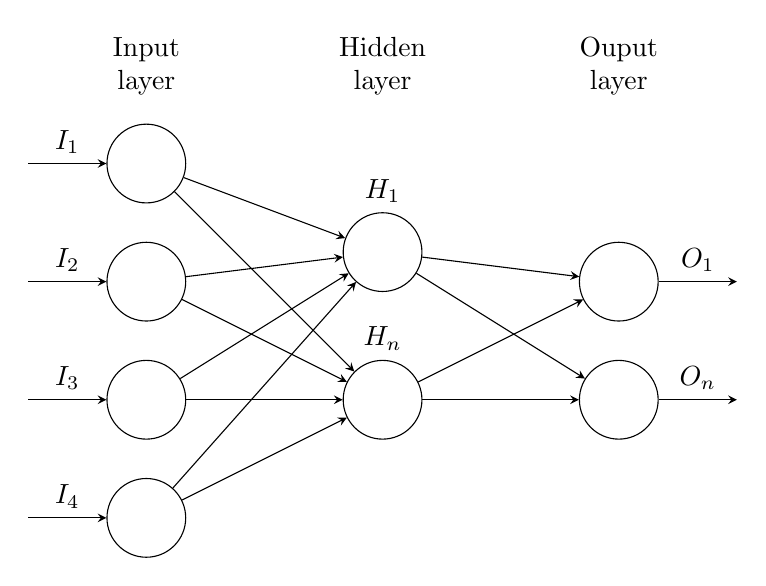
\begin{tikzpicture}[x=1.5cm, y=1.5cm, >=stealth]
		
		\foreach \m/\l [count=\y] in {1,2,3,4}
		\node [every neuron/.try, neuron \m/.try] (input-\m) at (0,2.5-\y) {};
		
		\foreach \m [count=\y] in {1,2}
		\node [every neuron/.try, neuron \m/.try ] (hidden-\m) at (2,2-\y*1.25) {};
		
		\foreach \m [count=\y] in {1,2}
		\node [every neuron/.try, neuron \m/.try ] (output-\m) at (4,1.5-\y) {};
		
		\foreach \l [count=\i] in {1,2,3,4}
		\draw [<-] (input-\i) -- ++(-1,0)
		node [above, midway] {$I_\l$};
		
		\foreach \l [count=\i] in {1,n}
		\node [above] at (hidden-\i.north) {$H_\l$};
		
		\foreach \l [count=\i] in {1,n}
		\draw [->] (output-\i) -- ++(1,0)
		node [above, midway] {$O_\l$};
		
		\foreach \i in {1,...,4}
		\foreach \j in {1,...,2}
		\draw [->] (input-\i) -- (hidden-\j);
		
		\foreach \i in {1,...,2}
		\foreach \j in {1,...,2}
		\draw [->] (hidden-\i) -- (output-\j);
		
		\foreach \l [count=\x from 0] in {Input, Hidden, Ouput}
		\node [align=center, above] at (\x*2,2) {\l \\ layer};
		
		\end{tikzpicture}
		\\
		This particular network takes an input vector of size $4$ and has output vectors of size $2$. This can be deduced from the fact that the \textit{input layer} of the network has $4$ nodes, while the \textit{output layer} contains $2$ nodes. Every node has its own floating-point value between $0$ and $1$, similar to the electric charge of the neurons in the human brain. In between the input- and output layers, there can be multiple so-called \textit{hidden layers}.
		
		When computing the output vector for a given input vector, the procedure is as follows: set the values of the nodes in the input layer equal to the values in the input vector. Then, the values of the other nodes are computed layer by layer. For each node in a layer, take all the incoming connections from the previous layer (represented by the arrows in the graph). Each of these connections has some number associated with it representing the 'thickness' of the connection between the two 'neurons', called the \textit{weights}. Take the values of all the nodes in the previous layer connected to the first node and multiply them with their respective weights and add up the results. Then, normalize the result between $0$ and $1$ by running it through a special mathematical function, usually the sigmoid function, which is defined as:
		\begin{equation*}
		\sigma(z) = \frac1{1+e^{-z}}
		\end{equation*}
		The value which the sigmoid gives back is the value of the node.
		
		For example, let's say that in the example network we have$I_1=0,5$, $I_2=0,8$, $I_3=0,1$ and $I_4=0,1$  and for the weights $w_{I_1,H_1}=2$, $w_{I_2,H_1}=0,3$, $w_{I_3,H_1}=0.7$ and $w_{I_4,H_1}=5$. In order to compute the value of $H_1$, first multiply the values of $I_1$, $I_2$, $I_3$ and $I_4$ by their respective weights and add them all up:
		\begin{equation*}
		0,5\cdot 2 + 0,8\cdot 0,3 + 0,1\cdot 0,7 + 0,1\cdot 5 = 1,81
		\end{equation*}
		Finally, run it through the sigmoid function, giving the value of $H_1$ as $\sigma(1,81)\approx 0,86$.
		
		The original inspiration behind neural networks was the human brain. Later, it was proven by George Cybenko \cite{cybenko} that neural networks with enough layers and correct weights could approximate almost any function, meaning that artificial neural networks could theoretically be trained to compute anything, given all the necessary input. It should be remarked that in practice this is impossible, since it requires an enormous amount of time and resources to find the right weights for large networks.
		
		When discussing the process of finding the right weights for a network (this process is called \textit{training}), it will prove useful to have a mathematical model of a neural net. The usual model is as follows:
		\begin{itemize}
			\item Every layer of the network is assigned a number from $0$ to $L$, where the input layer 			has index $0$, the output layer has index $L$ and the hidden layers have indices $1,2,					\ldots,L-2,L-1$.
			\item For any layer $l$, the amount of nodes in that particular layer is called $n_l$.
			\item For any layer $l$, we have $o^l_i$ as the value of the $i$'th node in the layer, with 			$1\le i\le n_l$.
			\item The weight of a connection between nodes $o^l_i$ and $o^{l+1}_j$ is represented by 				$w^l_{i,j}$. When two nodes in consecutive layers are not connected, simply take their 				weight equal to $0$.
		\end{itemize}
		Now, a single formula can be used to characterize the entire network. For all $0\le l\le L-1$ and all $1\le i\le n_l$ we have:
		\begin{equation*}
		o^{l+1}_i = \sigma\left(\sum_{j=1}^{n_{l}}o^{l}_j\cdot w^{l}_{j,i}\right)
		\end{equation*}
		
		\subsection{Convolutional neural networks}
		A more advanced version of the neural net, is the so-called convolutional neural network. These types of networks were first created by Yann LeCun \cite{lecun} in 1998. They were designed especially 	for image recognition and differ from classical neural networks quite drastically. First, some essential concepts unique to CNNs (acronym for Convolutional Neural Network) will be discussed, followed by a full overview of a standard CNN.
		
		\subsubsection{Features}
		Features are little pieces that are used to recognize a larger picture. For example if a neural net needs to recognize a cross-shape, the features will be two diagonal lines, crossing each other at a right angle. By dividing the process of recognition up into small subprocesses which detect certain features, the possibility space is reduced, leading to better performance of the AI.
		
		\subsubsection{Convolution} \label{convolution}
		Feature detection is performed by an operation called \textit{convolution}. For simplicity's sake, convolution will only be explained for gray-scale images, though it can also be used on colored images. Say we have a very small image of a white cross on a black background. When represented as a matrix of pixel values, the image looks like this:
		\begin{equation*}
		\begin{pmatrix}
		1 &0 &0 &0 &0 &1\\
		0 &1 &0 &0 &1 &0\\
		0 &0 &1 &1 &0 &0\\
		0 &0 &1 &1 &0 &0\\
		0 &1 &0 &0 &1 &0\\
		1 &0 &0 &0 &0 &1
		\end{pmatrix}
		\end{equation*}
		Where gray-scale pixels are represented by floating-point numbers between $0$ and $1$, $0$ being black and $1$ being white. Feature detection through convolution consists of choosing an appropriate small matrix, called the \textit{kernel}. The kernel is then shifted over the original image and a new, slightly smaller image is created. For every point in the new image, the kernel is places onto the old image, such that the center value of the kernel is right above the associated value of the original image. Then each kernel value is multiplied with the image pixel value directly 'beneath' it. The results are added up and this is the new pixel value. Convolution is represented by the $*$-operator. For example:
		\begin{equation*}
		\begin{pmatrix}
		1 &0 &0 &0 &0 &1\\
		0 &1 &0 &0 &1 &0\\
		0 &0 &1 &1 &0 &0\\
		0 &0 &1 &1 &0 &0\\
		0 &1 &0 &0 &1 &0\\
		1 &0 &0 &0 &0 &1
		\end{pmatrix} * \begin{pmatrix}
		1 &-1 &-1\\
		-1 &1 &-1\\
		-1 &-1 &1
		\end{pmatrix} = \begin{pmatrix}
		3 &1 &-3 &-3\\
		-1 & -3 & -3 &-3\\
		-3 &-3 &1 &-1\\
		-1 &-3 &-1 &3
		\end{pmatrix}
		\end{equation*}
		When the kernel is put in the top-left corner of the original image, all the $-1$-value are right above a $0$, while the $1$s in the kernel are right above other $1$s, giving a total sum of $3$. When the kernel is shifted one to the right, most kernel value are above a $0$, however, two $1$s in the kernel is above a $1$ in the original image and a single $-1$ in the kernel is right above a $1$ in the image, giving a value of $2\cdot 1+1\cdot -1=1$. The same process is repeated for the entire image. This example kernel detects diagonal lines from the top-left to the bottom-right. As can be seen, the highest values in the resulting image occur at points where the original image had such a line.
		
		\subsubsection{ReLu}\label{ReLu}
		Because pixels cannot have negative values and because of quite complex mathematical reasons, it is common practice to apply a Rectified Linear Unit (ReLu) to the result of the convolution. This means that all negative values are set to $0$. For example:
		\begin{equation*}
		\operatorname{ReLu}\begin{pmatrix}
		3 &1 &-3 &-3\\
		-1 & -3 & -3 &-3\\
		-3 &-3 &1 &-1\\
		-1 &-3 &-1 &3
		\end{pmatrix} = \begin{pmatrix}
		3 &1 &0 &0\\
		0 & 0 & 0 &0\\
		0 &0 &1 &0\\
		0 &0 &0 &3
		\end{pmatrix}
		\end{equation*}
		
		\subsubsection{Pooling}\label{pooling}
		Some features do not need extremely detailed images to be recognized. And since working with lower resolution images increases performance, a process called \textit{pooling} is used. The image is divided up into small pieces, usually $2\times 2$ pixels. Then these small pieces are all compressed to a single value. The most common forms of pooling are average pooling, where the average of all the pixel values inside each piece is taken and max pooling, where the maximum pixel value within each piece is taken. Because is vastly simplifies the mathematics later on, the choice has been made to use max pooling. The size of the small pieces the image is divided up into, is called the \textit{pooling kernel}. As an example, if max pooling with a $2\times 2$ kernel is applied to the image from before, we obtain:
		\begin{equation*}
		\operatorname{maxPool}\begin{pmatrix}
		3 &1 &0 &0\\
		0 & 0 & 0 &0\\
		0 &0 &1 &0\\
		0 &0 &0 &3
		\end{pmatrix} = \begin{pmatrix}
		3 &0\\
		0 &3
		\end{pmatrix}
		\end{equation*}
		
		
		\subsubsection{Training}
		The idea behind machine learning with convolutional neural networks, is to take a network structure and randomly initialize all the kernels. Then, a lot of already classified data is put trough the network. Since the correct output values are already known, it is possible to compute the \textit{error}, sometimes referred to as the \textit{cost}. Subsequently, the \textit{backpropagation algorithm} is used to compute how much each kernel influenced the error and by how much. This information is then used to slightly updating the kernels, making the network a tiny bit better at its task. Ultimately, this form of \textit{supervised learning} can lead to near-human or sometimes even super-human capabilities.
		
		The learning process will now be formalized by deriving a very general form of the backpropagation algorithm. Though specific instances of this algorithm were already known to the authors, the general form has been derived independently.
		
		First, some terminology must be introduced.
		\begin{itemize}
			\item The layers are enumerated $0$ to $L$, layer $0$ being the input layer and layer $L$ being the output layer.
			\item The neurons are enumerated per layer. $o_i^l$ is the value of the $i$'th neuron in the $l$'th layer.
			\item The activation function is named $f$.
			\item The kernel between the $i$'th neuron in the $l$'th layer and the $j$'th neuron in the $l+1$'th layer is denoted by $w_{i,j}^{l+1}$.
			\item The result of convolution and averaging in neuron $i$ of layer $l$ is called $x_i^l$, so that $o_i^l=f(x_i^l)$
			\item For any given input, the target value of the $i$'th node in the output layer is $t_i$.
		\end{itemize} 
		The usual definition of addition and subtraction of tensors will be used. $\circ$ will be the Hadamard product and $\otimes$ will be convolution. Exponentiation will be used with the Hadamard product. When summing over all neurons in a layer $l$, denote it as:
		\begin{equation*}
		\sum_{i\in l}o^l_i
		\end{equation*}
		
		For any given input, the error is defined as:
		\begin{equation*}
		E = \frac12\sum_{i\in L}\left(o^L_i-t_i\right)^2
		\end{equation*}
		The goal is to minimize the error and for that, the derivative,
		\begin{equation*}
		\frac{\partial E}{\partial w^l_{i,j}},
		\end{equation*}
		must be computed for each kernel $w^l_{i,j}$. If $E$ is seen as a function of $x_k^l$ for all $k\in l$, we can take the total derivative and arrive at:
		\begin{equation*}
		\frac{\partial E}{\partial w^l_{i,j}} = \sum_{k\in l}\left(\frac{\partial E}{\partial x^l_k}\cdot\frac{\partial x^l_k}{x^l_j}\right) = \frac{\partial E}{\partial x^l_j}\cdot \frac{\partial x^l_j}{\partial w^l_{i,j}}
		\end{equation*} 
		Where the second step is possible because $w^l_{i,j}$ only has an influence on $x^l_j$ and none of the other $x^l_k$ with $k\in l$. Now, $x^l_j$ is defined as:
		\begin{equation*}
		x^l_j = \sum_{k\in l-1}o^{l-1}_k\otimes w^l_{k,j}
		\end{equation*}
		We conclude:
		\begin{equation*}
		\frac{\partial x^l_j}{\partial w^l_{i,j}} = \frac{\partial}{\partial w^l_{i,j}}\left(\sum_{k\in l-1}o^{l-1}_k\otimes w^l_{k,j}\right) = \frac{\partial(o^{l-1}_i\otimes w^l_{i,j})}{\partial w^l_{i,j}} = o^{l-1}_i
		\end{equation*}
		Defining $\delta^l_j = \frac{\partial E}{\partial x^l_j}$ and filling in now yields:
		\begin{equation*}
		\frac{\partial E}{\partial w^l_{i,j}} = o^{l-1}_i\circ \delta^l_j
		\end{equation*}
		
		Suppose that $l=L$. This yields:
		\begin{equation*}
		\delta_j^l = \frac{\partial}{\partial x^l_j}\left(\frac12\sum_{i\in L}\left(o^L_i-t_i\right)^2\right) = \frac{\partial(\frac12(f(x^l_j)-t_j)^2)}{\partial x^l_j} = (o^l_j-t_j)\circ f'(x^l_j)
		\end{equation*}
		by the chain rule. For all other $l$, we can take $E$ as a function of $x^{l+1}_k$ for all $k\in l+1$ and take the total derivative for tensors:
		\begin{equation*}
		\delta^l_j = \sum_{k\in l+1}\left(\frac{\partial E}{\partial x^{l+1}_k}\otimes rot_{180}\left(\frac{\partial x^{l+1}_k}{\partial x^l_j}\right)\right) = \sum_{k\in l+1}\left(\delta^{l+1}_k\otimes rot_{180}\left(\frac{\partial x^{l+1}_k}{\partial x^l_j}\right)\right)
		\end{equation*}
		and:
		\begin{align*}
		\frac{\partial x^{l+1}_k}{\partial x^l_j} &= \frac{\partial}{\partial x^l_j}\left(\sum_{i\in l}o^l_i\otimes w^{l+1}_{i,k}\right)\\
		&=\frac{\partial(o^l_j\otimes w^{l+1}_{j,k})}{\partial x^{l}_j}\\
		&=\frac{\partial(f(x^l_j)\otimes w^{l+1}_{j,k})}{\partial x^{l}_j} =f'(x^l_j)\circ w^{l+1}_{j,k}
		\end{align*}
		finally yielding:
		\begin{equation*}
		\delta^l_j = \begin{cases}
		f'(x^l_j)\circ (o^l_j-t_j)&\text{ if $l=L$}\\
		f'(x^l_j)\circ\sum_{k\in l+1}\left(\delta^{l+1}_k\otimes rot_{180}(w^{l+1}_{j,k})\right)&\text{ otherwise}
		\end{cases}
		\end{equation*}
		and
		\begin{equation*}
		\frac{\partial E}{\partial w^l_{i,j}} = o^{l-1}_i\circ \delta^{l}_j
		\end{equation*}
		Now, the weights can be updated by choosing a small learning value $\mu$ and taking:
		\begin{equation*}
		w^{l}_{i,j}\mapsto w^{l}_{i,j}-\mu\frac{\partial E}{\partial w^l_{i,j}}
		\end{equation*}
		
		
		\subsection{The network}
		(We haven’t finished this part for now, it will follow as soon as possible)
		
		\section{The code explained}
		
		\subsection{The FileHandler class} \label{Filehandler}
		This is a very basic class purely used to be able to save and load data. It has the following methods:
		\begin{lstlisting}
		public static void saveParameters(String file_path, String file_content) 	
		public static String loadParameters(String file_path)
		
		public static BufferedImage loadImage(String img_path,  int width, int height)
		public static void saveImage(BufferedImage buf_img, String save_path)
		\end{lstlisting}
		The first two are simply used to save a string to a file and load it again. For this they only need a file path given. The last two are used for converting an image to a BufferedImage and the other way around. Using this, edited images can be saved to and loaded from a given file path.
		.
		\pagebreak
		
		\subsection{The Preprocessing class} \label{preprocess}
		This class converts the loaded images to the size they need to be in order to be able to be as input to the network.
		It has the following fields:
		\begin{lstlisting}
		private static final int IMAGE_WIDTH = 256;
		private static final int IMAGE_HEIGHT = 256;
		\end{lstlisting}
		
		These two constants give the size the images must be in order for them to be accepted as input for the network, which is 256x256
		
		The Preprocessing class has these methods:
		\begin{lstlisting}
		public static Tensor preproces(BufferedImage input_image)
		private static BufferedImage scale(BufferedImage input_image, double scale)
		private static BufferedImage crop(BufferedImage input_image, int start_x, int start_y, int width, 		int height)
		\end{lstlisting}
		The preproces method converts a BufferedImage to a Tensor, this will be explained in the next section, using the other private methods scale and crop.
		The scale method scales the image so that one of the dimensions is correct after which the crop method will cut off the sides to make the other dimension fit as well. After which one of the Tensor methods is used to convert this image to a Tensor that can later be used by the AI. 	
		\pagebreak
		
		\subsection{The Tensor class} \label{Tensor}
		As discussed before, a convolutional neural network relies heavily on two-dimensional data. After, all the input to the network consists of three two-dimensional arrays of red, green and blue pixel values respectively. It would therefore be sufficient to utilize Javas' built-in two-dimensional arrays.
		
		However, as stated earlier, the possibility of using the AI for other things than facial recognition is a very real one. These other applications may require higher dimensional data structures, something to keep in mind when designing the AI.
		
		This is why it was decided to design and build a custom data structure capable not only of containing multi-dimensional data, but also of performing certain transformations essential to the network, such as convolution, or ReLu. This custom data structure is the \textit{Tensor} class.
		
		The fields of the Tensor class are:
		\begin{lstlisting}
		public int dimension;
		public int[] lengths[];
		
		private int total_data_length;
		private int[] index_products;
		private float[] data;
		\end{lstlisting}
		The \textit{dimension} field contains the dimension of the Tensor. A zero-dimensional tensor is basically a float, a one-dimensional Tensor is a vector, a two-dimensional Tensor is a matrix and so on.
		
		\textit{lengths} contains what could be called the 'shape' of the Tensor. For a zero-dimensional Tensor this array is empty. In a one-dimensional Tensor, it contains the width, in a two-dimensional Tensor the width and height, in a three-dimensional Tensor the width, height and depth and so on.
		
		The actual data is stored in \textit{data} and the total amount of data (i.e., the length of the \textit{data} array) is contained in \textit{total\_data\_length}. As  will notice, all data is stored in a serialized form. \textit{index\_products} will be looked at in more depth later.
		
		The methods of the Tensor class are:
		\begin{lstlisting}
		public Tensor(int... lengths);
		public Tensor(float[] data, int... lengths);
		public Tensor(float lower, float upper, int... lengths);
		public Tensor(Tensor[] tensors) throws DimensionException;
		public void become(Tensor tensor);
		
		public float get(int... indices);
		public void set(float value, int... indices) throws DimensionException;
		public int getSerializedDataIndex(int... indices) throws DimensionException;
		public float[] getSerializedData();
		
		public void flatten();
		public void ReLu();
		public void convolveWith(Tensor kernel) throws DimensionException;
		public void maxPool(int... poooling_lengths) throws DimensionException;
		public void reduceDimension() throws DimensionException;
		
		public static Tensor add(Tensor ...tensors) throws Exception;
		public static Tensor scalarMult(float val, Tensor tensor);
		public static Tensor subtract(Tensor t1, Tensor t2) throws Exception;
		public static Tensor Hadamard(Tensor t1, Tensor t2) throws Exception;
		public static Tensor invertMaxPooling(Tensor result, Tensor propagation_widener, int ...pooling_lengths) throws DimensionException;
		public static Tensor rot180(Tensor tensor) throws DimensionException;
		\end{lstlisting}
		The first five methods all have something to do with making Tensors. The first four are constructors and the \textit{become} method makes \textit{this} become its \textit{tensor} argument, something which is useful in the other methods.
		
		The next four methods are very general methods used for working with Tensors. The \textit{get} and \textit{set} methods speak for themselves and the \textit{getSerializedData} method simply returns the Tensors \textit{data} field. The really interesting one is \textit{getSerializedDataIndex}. 	
		
		\subsubsection{getSerializedDataIndex}
		As stated earlier, the Tensor class uses a simple array for data storage under the hood, but when accessing data, a user specifies 'coordinates', or 'indices' as they are called in most method parameters. These coordinates need to be converted to a single index in the \textit{data} array and that is what the \textit{getSerializedDataIndex} is for. Its definition is:
		\begin{lstlisting}
		public void getSerializedDataIndex(int... indices) throws DimensionException
		{
		if(indices.length != this.dimension)
		{
		throw new DimensionException("the amount of indices must be equal to the dimension");
		}
		
		int index = 0;
		for(int i = 0; i < this.dimension; i++)
		{
		index += indices[i] * this.index_products[i];
		}
		return index;
		}
		\end{lstlisting}
		First, it is checked if the right amount of 'coordinates', or \textit{indices} has been used. If not, a custom exception is thrown. What happens next needs to be explained in more detail.
		
		As an example of how the index is computed, take a look at a two-dimensional Tensor, which can simply be seen as a matrix. Say we have some $3\times 3$ matrix and want to store it in a serialized manner. The most obvious way to do this, is to concentrate all rows of the matrix into a single array. For example:
		\begin{equation*}
		\begin{bmatrix}
		a &b &c\\
		d &e &f\\
		g &h &i
		\end{bmatrix}\stackrel{\text{serialize}}{\longrightarrow} [a,b,c,d,e,f,g,h,i]
		\end{equation*}
		Suppose we want to find the index of the element at $(1,1)$. Since the matrix is zero-indexed this is the element $e$. The index of the first element of the first row is $0$, the index of the first element of the second row is $3$ and the index of the first element of the third row is $6$. So the index of $(0,1)$ is $3$. Because of the way the serialized array was constructed, the next element will be the element to the right of $(0,1)$, also known as $(1,1)$. It follows that the index of $(1,1)$ is $3\cdot 1 + 1 = 4$.
		
		In general, if we have some $m\times n$ matrix, the serialized index of some element with indices $(a,b)$ is equal to $a+b\cdot m$. It turns out that in a three-dimensional $m\times n\times k$ Tensor, the serialized index of an element with indices $(a,b,c)$ is equal to $a+m\cdot b+m\cdot n\cdot c$. The concept can be further generalized to Tensors of any dimension. Say we have some $m_1\times m_2\times\ldots\times m_n$ Tensor of dimension $n$. Now, the serialized index of any element with indices $(a_1,a_2,\ldots,a_n)$ is equal to:
		\begin{equation*}
		\sum_{i=1}^{n}a_i\left(\prod_{j=1}^{i-1}m_j\right).
		\end{equation*}
		The numbers
		\begin{equation*}
		\prod_{j=1}^{i-1}m_j
		\end{equation*}
		are computed in the constructor. These are the \textit{index\_products} seen before, when discussing the fields of the Tensor class (remark: Notice that for $i=1$,  a product from $j=1$ to $j=0$ is obtained. This 'empty product' is defined as $1$). Multiplying with these 'index products' and adding everything together is precisely what is done in the \textit{getSerializedDataIndex} method.
		
		\subsubsection{flatten and ReLu}
		Since all the remaining Tensor methods are of critical importance for the neural network, every one of them will be discussed briefly. First, the \textit{flatten} method. As mentioned in the explanation of convolutional neural nets, the multiple feature maps which form the input of every single hidden node are combined at that hidden node. To be specific, their average is taken. The way this is done, is by combining all incoming two-dimensional feature maps into a single three-dimensional Tensor. This is done with the
		\begin{lstlisting}
		public Tensor(Tensor[] tensors) throws DimensionException;
		\end{lstlisting}
		constructor. Then, the tensor is ‘flattened’ by replacing all 'rows' with their average. An example on a two-dimensional Tensor would be:
		\begin{equation*}
		\begin{bmatrix}
		a &b &c\\
		d &e &f\\
		g &h &i
		\end{bmatrix}\stackrel{\text{flatten}}{\longrightarrow}
		\begin{bmatrix}
		\frac13(a+b+c)\\
		\frac13(d+e+f)\\
		\frac13(g+h+i)
		\end{bmatrix}.
		\end{equation*}
		Since the Tensor can be seen as an array of 'rows', just as it can be seen it as an array of values when it is serialized, all that is needed in order to pretend we are working in a matrix is a single nested loop.
		
		The \textit{ReLu} method simply sets all negative data values to $0$. This hasn't got anything to do with indices or the dimension of the Tensor, so \textit{ReLu} simply iterates over the \textit{data} field.
		
		\subsubsection{convolveWith and maxPooling} \label{convolveWith}
		The workings of convolution and max pooling have been discussed at length in the chapter on the theory behind convolutional neural networks, so rather than focusing on what convolution and max pooling are, a close look will be taken at one of the programming challenges encountered when writing both methods.
		
		Both the \textit{convolveWith} and \textit{maxPooling} methods need to iterate over all data in the Tensor. Not only that, they also need to know the where the value they are currently working with is located in the Tensor, since both methods need to know about the neighbours of the value they are currently working with. This means that the naive approach of a simple for-loop iterating over the \textit{data} field won't work. Nested for-loops are out of the picture as well, since the amount of nested for-loops needed, would be equal to the dimension of the Tensor.
		
		Instead, these two methods are combined. A single for loop will iterate over the \textit{data} field and meanwhile, the 'coordinates' of the current value will be kept track of in an array called \textit{indices}. This way, the \textit{get} method can be used to retrieve the values of neighbours and other 'close-by' elements:
		\begin{lstlisting}
		//This array will hold the 'position' within the tensor
		int[] indices = new int[this.dimension];
		for(int i = 0; i < this.dimension; i++)
		{
		//we're starting in the 'top-left corner'
		indices[i] = 0;
		}
		
		for(int i = 0; i < this.total_data_length; i++)
		{
		//here everything that needs to be done is done 
		
		//update indices
		indices[0]++;
		for(int j = 0; j < this.dimension - 1; j++)
		{
		if(indices[j] == this.lengths[j])
		{
		indices[j] = 0;
		indices[j+1]++;
		}
		}
		}
		\end{lstlisting}
		First, the \textit{indices} array is initialized. Then the main for-loop iterates over all Tensor data. At the end of each iteration the indices are updated. Although this process is hard to describe in general, describing it in a three-dimensional Tensor will most likely foster an understanding of the general process.
		
		Imagine for a moment a cuboid, divided up into small square cells, with each cell containing some floating-punt number. This represents the \textit{data} array of a three-dimensional Tensor. Let's iterate through the array. Start in the top-left corner (the \textit{indices} array is initialized). Now, every iteration, a single step is performed towards the right. (the first element of \textit{indices} is increased by one). Now, check whether the edge of the cuboid and the end of the current row has been reached. If so, go back to the left and move a single cell forward, such that we are now at the beginning of the next row (the first iteration of the for-loop with index $j$). If not only the last cell in a row has been reached, but also the last row in a 'slice', move all the way back and one cell down (the second iteration of the for-loop with index $j$). It isn’t needed to check whether or not the last index has reached its maximum (the upper bound in the for-loop with index $j$ is \textit{this.dimension-1} instead of \textit{this.dimension}), since if this is the case, we have arrived at the last cell of the cuboid and we are done.
		
		The above is an explanation for how updating \textit{indices} works in three dimensions. In the code snippet presented earlier, this process is generalized to any dimension. Perhaps these higher-dimensional cases can be compared to continuously adding $1$ to an integer. Starting with $0$, this yields the sequence:
		\begin{equation*}
		0\to1\to 2\to 3\to 4\to 5\to 6\to 7\to 8\to 9
		\end{equation*}
		When $1$ is added once more, the last digit has already reached its maximum value of $9$ and turns to its minimum value of $0$, while the second-to-last digit increases by $1$ and becomes $1$, so the next number in the sequence is $10$. The \textit{indices} can be viewed as the digits of a number which keeps increasing by $1$. The only difference is, that in the example, each digit has a maximum value of $9$, while in the code snippet, the 'digit' in the $i$'th place has a maximum value of \textit{this.lengths[i]-1}, so instead of checking whether the digit in the $i$'th place is equal to $10$ (which means it should be set to $0$, since $9$ is its maximum value), it is checked whether \textit{indices[i]} is equal to \textit{this.lengths[i]}.
		
		Apart from the this difficulty regarding iteration, both methods are fairly straightforward to implement. It should be remarked that the described iteration technique is used twice in both \textit{convolveWith} and \textit{maxPooling}. In \textit{convolveWith}, we first iterate over all Tensor data. Then, for each Tensor data value, we iterate over the kernel, in order to compute a single value in the resulting Tensor.
		
		In the \textit{maxPooling} method,first a smaller Tensor is created to store the result. Then, we iterate over this new Tensor and for each value in the result, we iterate over its associated 'neighbourhood' in the original Tensor, while keeping track of the maximum, so that the value can be set to this maximum later.
		
		\subsubsection{reduceDimension}
		As data passes through the convolutional neural net, the Tensors keep getting smaller due to pooling. As input, there are three large two-dimensional Tensors representing the red, green and blue channels of the input image. This means that the input nodes of the network contain Tensors of dimension $2$. However, the output nodes contain simple numerical values, or Tensors of dimension $0$. Somewhere in the network the dimension of the Tensors needs to be reduced.
		
		Since the Tensors cannot get larger as they pass through the net, only smaller, the dimension of a Tensor can be reduced as soon as one of the dimensions becomes redundant. For example, if, at some point, a two-dimensional Tensor of width $1$ is obtained, its width will be less than or equal to $1$ for the rest of the net. Two-dimensional Tensors with width $1$ are basically one-dimensional Tensors. Since one-dimensional Tensors contain slightly less data than two-dimensional Tensors, it is best to actually reduce the dimension.
		
		This is what \textit{reduceDimension} is for. It iterates through \textit{this.lengths}, finding all 'lengths' equal to $1$, meaning that that particular dimension can be 'removed'. It then creates a Tensor of the appropriate dimension and moves all data to it, after which the Tensor \textit{becomes} that new Tensor.
		
		\subsection{Tensor arithmetic}
		The next four methods all have something to do with basic Tensor arithmetic. The \textit{add} method simply adds one or more Tensors together element-wise. The \textit{scalarMult} method multiplies all entries of a given Tensor with a given floating-point number. These two methods are combined in the \textit{subtract} method, which returns the element-wise difference of two given Tensors.
		
		Finally, the \textit{Hadamard} method returns the Hadamard (element-wise) product of two given Tensors. All the arithmetic functions check whether their input Tensors are of the same size. If not, they will throw an Exception.
		
		\subsection{invertMaxPooling and rot180}
		The final two methods are \textit{invertMaxPooling} and \textit{rot180}. Both are used in the backpropagation algorithm. When the \textit{maxPooling} method is applies to a Tensor, it turns this Tensor into a smaller Tensor and returns a so-called 'propagation-widener'. When this propagation-widener and the new Tensor are fed into \textit{invertMaxPooling}, the method returns the new Tensor with its values in the original place. For example, if max pooling is applied like this:
		\begin{equation*}
		\begin{pmatrix}
		0 &1 &2 &3\\
		4 &5 &6 &7\\
		8 &9 &10 &11\\
		12 &13 &14 &15
		\end{pmatrix}\stackrel{maxPooling}{\longrightarrow} \begin{pmatrix}
		5 & 7\\
		13 &15
		\end{pmatrix}
		\end{equation*}
		then \text{invertMaxPooling} does the following:
		\begin{equation*}
		\begin{pmatrix}
		5 & 7\\
		13 &15
		\end{pmatrix} \stackrel{invertMaxPooling}{\longrightarrow}\begin{pmatrix}
		0 &0 &0 &0\\
		0 &5 &0 &7\\
		0 &0 &0 &0\\
		0 &13 &0 &15
		\end{pmatrix}
		\end{equation*}
		Here, the propagation-widener would have looked like this:
		\begin{equation*}
		\begin{pmatrix}
		0 &0 &0 &0\\
		0 &1 &0 &1\\
		0 &0 &0 &0\\
		0 &1 &0 &1\\
		\end{pmatrix}
		\end{equation*}
		
		The \textit{rot180} method rotates a Tensor $180^\circ$ in all directions. For example:
		\begin{equation*}
		\begin{pmatrix}
		0 &1 &2 &3\\
		4 &5 &6 &7\\
		8 &9 &10 &11\\
		12 &13 &14 &15
		\end{pmatrix}\stackrel{rot180}{\longrightarrow} \begin{pmatrix}
		15 &14 &13 &12\\
		11 &10 &9 &8\\
		7 &6 &5 &4\\
		3 &2 &1 &0
		\end{pmatrix}
		\end{equation*}
		Both these methods are used in the backpropagation algorithm.
		
		\subsection{The Training class}
		The training class will be responsible for the training of the AI. This class will choose the pictures with which the AI will be trained.
		
		This class has the following fields
		\begin{lstlisting}
		private int number_of_subjects;
		private int number_of_pictures;
		private String image_path;
		Random random = new Random();
		\end{lstlisting}
		
		The integers store amounts for the random number generator which is also made here, the String stores the path to the data which things can be added to later on, in order to get a full path to the image.
		
		This class has the following methods:
		\begin{lstlisting}
		public void train(int amount_of_runs);
		private Tensor loadTrainingSet(String path);
		private String getNextPath(String subject);
		
		public void setImagePath(String path);
		public void setNumberOfTestSubjects(int number);
		public void setNumberOfPictures(int number);
		\end{lstlisting}
		
		The last three methods are setters for the previously mentioned fields. The first three methods are the methods that actually do the first part of training, getting the required tensors and the desired output.
		
		In the train() method it is determined by a 'coin flip' whether the two pictures will be from the same person or from two random persons. With this done, the getNextPath() will construct a path to a picture from the given subject and then loadTrainingSet() will load this image and convert it to a Tensor using the preprocess(\ref{preprocess}) and Filehandler(\ref{Filehandler}) classes.
		
		\pagebreak
		
		\subsection{The ConvolutionalNeuralNetwork class}
		This class creates the network and allows us to perform certain actions like back propagation on the network. It makes use of the KernelLayer class and the NeuronLayer class, which will be explained in the next two sections.
		
		This class has a lot of fields declared at the start:
		\begin{lstlisting}
		public static final int CONV_NET_OK = 0;
		public static final int APPEND_ERROR = 1;
		public static final int DELETE_ERROR = 2;
		public static final int SIZE_ERROR = 3;
		public static final int DIMENSION_ERROR = 4;
		
		private ArrayList<NeuronLayer> neuron_layers;
		private ArrayList<KernelLayer> kernel_layers;
		
		private int neuron_layer_count;
		private int kernel_layer_count;
		
		private int neuron_in_count;
		private int neuron_out_count;
		
		private int dimension_in;
		private int dimension_out;
		
		private int[] output_lengths;
		\end{lstlisting}
		
		Most of these speak for themselves. The first constant are error codes used by this class. Then two Arraylists are declared, one for the kernel layers and one for the neuron layers. The last fields are variables that will be used to check if two layers 'fit' on each other.
		
		This class contains the following methods:
		\begin{lstlisting}
		public ConvolutionalNeuralNetwork(NeuronLayer input_layer);
		
		public int addNeuronLayer(NeuronLayer layer);
		public int addKernelLayer(KernelLayer layer);
		
		public int removeLastLayer();
		public Tensor[] process(Tensor[] input_data) throws Exception;
		public void backpropagate(Tensor[] input, Tensor[] desired_output) Throws exception;
		\end{lstlisting}
		
		The first one is the constructor of the network and the second and third one are used to add layers to this network. These two methods just check if everything matches like the amount of connections and then they are added to the network.
		
		The \textit{removeLastLayer} function will check if there is more than one layer, as the last one is the input and can't be deleted, and then it will delete this layer and update all the variables for the layer before it, so the checks to see if two layers match will still work.
		
		The \textit{process()} function will use the \textit{input\_data} and let it go through each of the neuron and kernel layers using their process functions and then return this processed data. 
		
		
		
		\pagebreak
		\subsection{The NeuronLayer class}
		This class will be used to create the neuron layers in the network, these layers will be use ReLu(\ref{ReLu}) and Pooling(\ref{pooling}) on the data and then send it through further. These two functions are programmed in the Tensor class and are there explained as well(\ref{Tensor})
		
		This class has the following fields:
		\begin{lstlisting}
		public int neuron_count;
		
		public int dimension_in;
		public int dimension_out;
		
		public int[] input_lengths;
		public int[] output_lengths;
		
		public int[] pooling_lengths;
		
		public Tensor[] neuron_data;
		
		public Tensor[] propagation_wideners;
		public Tensor[] delta_tensors;
		public Tensor[] relu_derivative;
		\end{lstlisting}
		
		The first five are data states what the layer looks like, these properties will be checked by the network to see if it can fit this layer on the previous layer. The \textit{pooling\_lengths} says how big the pooling will be, this will be explained later. The \textit{neuron\_data} speaks for itself. The last three fields are used for the backpropagation.
		
		The methods of this class are:
		
		\begin{lstlisting}
		public NeuronLayer(int neuron_count, int[] input_lengths, int[] pooling_lengths) throws 				DimensionException, NumericalException;
		public void process(Tensor[] input) throws DimensionException;
		\end{lstlisting}
		
		The first method is the constructor and checks if all the given variables will work, if this is not the case specific Dimension and Numerical exceptions will be thrown.
		
		Then the \textit{process()} function. This will be called by the network to actually process data. For the neuron layers this means performing pooling and ReLu. These functions are already explained in (\ref{Tensor}).
		
		\pagebreak
		\subsection{The KernelLayer class}
		This class will create the Kernel layers that connect the neuron layers.
		
		The fields are:
		\begin{lstlisting}
		public int dimension;
		
		public int neuron_in_count;
		public int neuron_out_count;
		
		private int[] kernel_lengths;
		public Tensor[][] kernels;
		\end{lstlisting}
		
		These fields give the data needed to create a random kernel and to check if loaded kernels actually fit. The last one \textit{Tensor[][] kernels} contains all of the kernel data once it is loaded.
		
		Then the methods of the class:
		\begin{lstlisting}
		public KernelLayer(int[] kernel_lengths, int neuron_in_count, int neuron_out_count, float lower, 		float upper) throws DimensionException;
		public KernelLayer(Tensor[][] kernels) throws Exception;
		public Tensor[] process(Tensor[] input_data) throws Exception;
		\end{lstlisting}
		
		The first one is the constructor for generating kernels randomly , the second one is the constructor for when it is loaded from a file.
		
		Here there is a \textit{process()} again to actually process the data. This one is a bit more complicated than the previous ones though. First there are checks for the dimensions and lengths of the input to see if they match the requirements. If all the checks are completed they will actually start processing using the following code:
		\begin{lstlisting}
		for(int i = 0; i < this.neuron_out_count; i++)
		{
		temp_tensors = new Tensor[this.neuron_in_count];
		for(int j = 0; j < this.neuron_in_count; j++)
		{				
		temp_tensors[j] = new Tensor();
		temp_tensors[j].become(input_data[j]);
		temp_tensors[j].convolveWith(this.kernels[j][i]);
		}
		output_data[i] = new Tensor(temp_tensors);
		output_data[i].flatten();
		}
		\end{lstlisting}
		For every output node we go through all the input nodes and send these through convolution using the convolveWith() method explained in \ref{convolveWith}. Once all the convolution has been completed, the method will attempt to reduce the size with flatten and then move on to the next output node. For more information on convolution, see \ref{convolution}.
		
		
		%--------------------------------------------------------------------------------------
		%Bibliography
		%--------------------------------------------------------------------------------------
		
		\begin{thebibliography}{99}
			\bibitem{camastra07}
			Camastra, F. \& Vinciarelli, A. (2007).\textit{Machine Learning for Audio, Image and Video 				analysis.} Dordrecht: Springer.
			
			\bibitem{deng13}
			Deng, L. \& Yu, D. (2013). \textit{Deep Learning: Methods and Applications.} Boston: Now 				Publisher Inc.
			
			\bibitem{karaaba16}
			Karaaba, M.F. (2016). \textit{Face recognition in low resolution images under small sample 				conditions with facepart detection and alignment.} Groningen: University of Groningen.
			
			\bibitem{andrews17}
			Andrews, T.M. (2017). \textit{China uses facial recognition software to crack down on toilet 			paper theft.} Consulted on 8 September 2017.
			
			\url{https://www.washingtonpost.com/news/morning-mix/wp/2017/03/21/china-uses-facial-					recognition-software-to-crack-down-on-toilet-paper-theft}
			
			\bibitem{dormehl14}
			Dormehl, D. (2014). \textit{Facial recognition: is the technology taking away your identity?} 			Consulted on 8 September 2017.
			
			\url{https://www.theguardian.com/technology/2014/may/04/facial-recognition-technology-					identity-tesco-ethical-issues}
			
			\bibitem{kuzovkin16}
			Kuzovkin, I. (2016). \textit{Deep Learning, Theory, history, state of the art \& practical 				tools.} Consulted on 8 September 2017.
			\url{http://ikuz.eu/2016/01/20/deep-learning-theory-history-state-of-the-art-practical-tools/}
			
			
			\bibitem{sapra16}
			Sapra, S. (2016). \textit{Artificial Neural Networks: State of the Art in Business 						Intelligence.} Consulted on 8 September 2017.
			
			\url{https://www.omicsonline.org/open-access/artificial-neural-networks-state-of-the-art-in-			business-intelligence-2151-6219-1000e107.pdf}
			
			\bibitem{gu}
			Gu, J. \& Wang, Z. (w.d.) \textit{Recent Advances in Convolutional Neural Networks.} Consulted 		on 8 September 2017.
			
			\url{https://arxiv.org/pdf/1512.07108.pdf}
			\bibitem{byford16}
			Byford, S. (2016). \textit{AlphaGo beats Lee Se-dol again to take Google DeepMind challenge 			series.} Consulted on 8 September 2017.
			\url{https://www.theverge.com/2016/3/12/11210650}
			
			\bibitem{foote17}
			Foote, K.D. (2017). \textit{A Brief History of Deep Learning.} Consulted on 8 September 2017
			\href{http://www.dataversity.net/brief-history-deep-learning/}{http://www.dataversity.net/				brief-history-deep-learning/}
			
			\bibitem{imageRecognition17}
			\textit{Image Recognition.} (2017). Consulted on 8 September 2017.
			\url{https://www.tensorflow.org/tutorials/image_recognition}
			
			\bibitem{3blue1brownNetwork}
			3Blue1Brown(2017). \textit{Neural Networks}. YouTube.
			\url{https://www.youtube.com/playlist?list=PLZHQObOWTQDNU6R1_67000Dx_ZCJB-3pi}
			
			\bibitem{cybenko}
			Cybenko, G. (1989). \textit{Approximation by Superpositions of a Sigmoidal Function}. 					Consulted on the 2'd of December 2017.
			\url{http://citeseerx.ist.psu.edu/viewdoc/download?doi=10.1.1.441.7873\&rep=rep1\&type=pdf}
			
			\bibitem{lecun}
			LeCun, Y. \&Bottou, L \&Bengio, Y\& Haffner, P. \textit{Gradient-Based Learning Applied to 				Document Recognition}. (1998). Consulted on the 2'd of December 2017.
			\url{http://yann.lecun.com/exdb/publis/pdf/lecun-01a.pdf}
		
		\bibitem{dataset}
		Nefian, A
		\textit{Georgia tech face database}. (1999). Consulted on the 23'rd of December 2017.
		\url{http://www.anefian.com/research/face_reco.htm}
	\end{thebibliography}
	
\end{document}





